\section{Implementation}
The problem with the ICN model, in IoT domain, lays in the nature of ICN with its data driven communication paradigm as described earlier. The data will only pass through the network if it has been requested. In a normal network approach, as in MQTT, the creator of a data can push it toward a user. This is impossible with the ICN paradigm. 
In order to achieve the same functionality, where the consumer retrieves the data from the sensor, an \textit{interest} request must have been initiated. Together with a one time subscription approach ICN could give the same functionality, as in MQTT, when data is produced periodically over time. To make such a system feasible, the performance of ICN has to be good enough so the system is not a bottleneck to itself. The optimal case is if the consumer could retreive the data as soon as it has been produced.\\\\
Through experimentations, this thesis tries to evaluate the performance and suitability described in earlier paragraph, of the ICN application CCN.\\\\
In the first experiment, in section 5, an evaluation regarding the latency performance is conducted . It covers differences in latency times between ping- and CCN peek requests between a consumer and a producer. The result provides arguments in favor of CCN, and they are later on used in the algorithm described in the second experiment.\\\\
The other experiment, covering an evaluation of the suitability using CCN can be found in section 6. It covers an analysis regarding the algortihm developed during the thesis and its performance from both a consumer and producers perspective. The algorithm tries to deliver the lowest possible latency, from the time the data has been produced until it is available to the consumer. 


\subsection{Setup}
The implementation of the experiments described in previous paragraphs consists of a combination of hardware and software. The setup is shown in figure \ref{fig:experiment_setup}, where the whole system consists of a computer, raspberry pi 3, slip radio and sensor. Together they communicate through various of protocols described both in section 2 and later on in this section. 
In order to provide logs and data for the experiments, the sensor is connected through USB to the computer. These logs are to verify that the system is correct. All communication between producer, the sensor, and the consumer, a CCN application running on Raspberry Pi, is made through a radio slip that is connected on a Raspberry Pi.

\begin{figure}\centering
	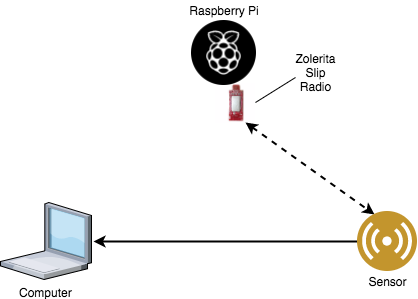
\includegraphics[width=0.7\textwidth]{figures/experiment_setup.png}
	%\caption{Star topology structure on the left, Peer-to-peer on the right. write where it is taken from?}
	\caption{Overview of the experimental setup. The sensor communicates with the radio slip mounted on a Raspberry Pi. Through the slip, a consumer application on the Raspberry is available to issue \textit{interest} request toward the sensor. The computer provides power to the sensor and in return it receives measurement logs.}
	\label{fig:experiment_setup}
\end{figure}
\subsubsection{Hardware}
The hardware setup used in this thesis consists of Texas Instrument CC2650 SensorTags, Zolertia Firefly and Raspberry Pi3. The sensortag produce sensor data that represent a IoT device. It communicate wirelessly with the Firefly-radio slip that is mounted on the Raspberry Pi3 which acts as a border gateway in this project. 

\paragraph{Texas Instrument CC2650 SensorTag}
The CC2650 sensortag is a wireless microcontroller developed by Texas Instruments \cite{CC2650}. The device is low cost, ultralow power device using the 2.4 Ghz radiofrequency to communicate with technologies such as 6LowPAN, Bluetooth and Zigbee. Due to its ultra low power consumption, the sensor can be powered by battery.
The CC2650 device contains a 32-bit ARM Cortex-M3 processor running at 48 Mhz, accompanied by 8 KB of cache and 20 KB of SRAM. It contains a total of 128 KB of programable flash memory, which can be used for different application system such as the Contiki-OS system. The sensor controller supports the measurement of different types of sensor data such as temperature readings, optical light values and more. 


\paragraph{Zolertia Firefly Slip radio}
The Firefly radio slip is developed by Zolertia \cite{Firefly}. The radio slip provides a network infrastructure for the IoT devices, enabling them to communicate efficiently through the air. The Firefly has great routing capabilities due to its support for several communication technologies, among them IEEE 802.15.4/6LowPAN and Zigbee. Another advantage using the Firefly is that it supports multiple types of frequency bands such as 2.4 GHz, 915- and 920 MHz band. Radio parameters such as modulation, data rate and transmission power are highly configurable.

\paragraph{Raspberry Pi 3}
The Raspberry Pi 3 is a single board computer developed by the Raspberry Pi Foundation \cite{RP3}. It contains components suchs as WIFI, several USB ports, 1 GB RAM and a quad core ARM processor among several other features. Due to its relativly high performance for a low price, it has become a popular developing tool used in projects at home, in school and for academic research.

\subsubsection{Software}
%There are some software running on the hardware in order to make everything to work. \todo{Rewrite all this. Arugment why we need this software on the hardware. Also describe very shortly the ccn application software. Also refer to background.}
The software setup used in this thesis consists of two CCN-lite applications \ref{CCN-LITE} \ref{yanqui}, Sparrow \ref{Sparrow} and Ping6. The CCN-lite software is used on the Linux platform and the portation described in previous section is used together with Contiki OS on the sensor node. To make them communicate with each other the Sparrow software creates a gateway together with the slip radio on the Raspberry Pi. This enables a reliable wireless communication channel between the router and the sensor.

\paragraph{Gateway CCN application}
%Has the possibility to send CCN interest requests and recieve data them. A peek latency tool has been developed to get the peek times.
%This application is sending the interest request through the gateway described in previous paragraph.
The CCN-lite application used on the border gateway has the possibility to send \textit{interest} message and recieve the \textit{data} for the request it has sent. To issue an \textit{interest} request, \textit{the ccn-lite-peek} application is used. It is an utility tool within the CCN-lite software that can create, encapsulate and send out requests on the radiolink and also recieve the corresponding data packet. A CCN peek application runs only one time, a request either receives the data or times out after a given time, thereafter the application terminates.\\\\
Additional functionality has, in this thesis, been added to this software to make it possible to calculate the latency for the difference between an \textit{interest} has been sent and when a response has been received. Throughout this thesis, CCN peek and peek is used interchangably in order to describe the round trip time from initiating a request to the time when that data has been received. 

\paragraph{Sensor CCN application}
The CCN application used for the sensors has a simple structure. Once the sensor has booted Contiki with CCN, it starts listening for incoming \textit{interest}-requests from the network and produces content objects.\\\\
When an \textit{interest} message is received at the sensor, a lookup in the cache will be performed to see if there is any matching content available. If there is a match in the \textit{content storage}, then a data message will be created with the content and sent int response towards the issuer. Otherwise, the \textit{interest} will be recorded in an entry in the \textit{pending interest table} and there is no response toward the user until the requested data has been produced.
An advantage is that this provides a possibility to ask for data that has not yet been produced. 
A consumer could potentially issue an \textit{interest} message a short time before the \textit{data} has been produced, which would firstly get the data directly to the user, and secondly reduce the latency on the network. 
\\\\
In every period a new content object is created. This object is cached into the \textit{content storage} to be retreived later on by an \textit{interest} request. There is also a lookup in the PIT to see if the newly created object already has an pending \textit{interest} request. If so, the object will be sent out towards the issuer and the request is to be considered consumed. Once the storage is full, the content will be removed from the \textit{content storage} in a FIFO-queue fashion.


\paragraph{Ping6}
The command ``live'' tool Ping6 is a utility software for linux systems which use the ICMPv6 protocol to send data over the network. In this thesis, it is used as a reference point for latency times in comparision to the CCN application.



\subsubsection{Communication flow between gateway and sensor}
In this experiment, a sensornode is connected via USB to a computer where one can monitor messages from the sensor. Through a 802.15.4 radio network, the sensor connect to a border router with Sparrow software running on it. All communication and message passing will be made between the the gateway and the sensornode over the 802.15.4 network. Above the 802.15.4 radio in the networking stack, data is encapsulated into 6LowPAN packets containing a full IPv6 header(of size 40 bytes). There are possibilites in Contiki-OS to compress the IP and networking headers by different strategies, but in in the implementation covered in this thesis, only the uncompressed 40 bytes IPv6 header will be considered. Thereafter the application data is encapsulated by either UDP or ICMPv6 as ther transportation protocol, both of those headers consist of 8 bytes. \todo{Behöver utvecklas för att ta med hela flödet, från application på GW till APP på sensor.}
\\\\

\subsubsection{Retrieve data}
In all experiments, the sensor node is connected via USB to a computer in order to retrieve measurement values. The live command tool TTY captures all these messages from the console that the sensor produces and make them readable for a user. 

After a few experiments, the result showed that the amount of information printed on the console had an impact on the latency.
After several iterations, a decision was made that there would be two versions of printing. One printing only a minimum of information and the other one printing all the essential information the evaluation needed. 

For verification purposes, the minimum printing sends information about whether an interest was responded or not. 
For the essential printing, information regarding \textit{interest} arrival times, \textit{data} departure times and other metric values essential to the result were added. As a consequence, there is a higher consumption of processing power at the sensor. This is shown in later measurement results when minimum printing takes one tick on the clock (1/128th seconds) longer.
